\documentclass{llncs}
\usepackage{makeidx}
\usepackage[spanish]{babel}
\usepackage[utf8]{inputenc}
\usepackage{amsmath}
\usepackage{url}
\usepackage{fancyvrb}
\usepackage[spanish]{babelbib}
\usepackage{graphicx}

%%%%%%%%%% Text with box
\usepackage{tikz}
\usetikzlibrary{shadows}

\newcommand{\raisedtext}[1]{%
  \begin{tikzpicture}
    [baseline=(X.base)]\node [drop shadow,fill=white,draw,very thin] (X) {#1};
  \end{tikzpicture}}
%%%%%%%%%%%%%%%%%%%

\graphicspath{ {img/} }

% \urldef{\mails}\path|{fbarrios,fjlopez}@fi.uba.ar| 

\newtheorem{definicion}{Definición} 

\begin{document}

\frontmatter

\title{Variantes de TextRank para la Generación de Resúmenes Automáticos}
\titlerunning{Variantes de TextRank} 

% \author{Federico Barrios, Federico López, Luis Argerich, Rosa Wachenchauzer}
% \institute{Facultad de Ingeniería, Universidad de Buenos Aires,\\
% Av. Paseo Colón 850, Ciudad Autónoma de Buenos Aires, Argentina\\
% \mails\\
% \url{http://ingenieria.uba.ar/}}

% \author{-}
% \institute{-}

\maketitle

\begin{abstract}
Este artículo describe el desarrollo y prueba de nuevas variantes del algoritmo
TextRank para la generación de resúmenes automáticos. Se describen las generalidades
del algoritmo TextRank en su versión original y las diferentes variantes
que fueron propuestas y probadas. Algunas de estas logran una mejora en
la performance del algoritmo de acuerdo a las métricas estándar para la evaluación de
resúmenes automáticos. 
\keywords{TextRank, resumen, automático}

\end{abstract}

\section{Introducción}
El proceso de generación de resúmenes automáticos consiste en extraer de un documento sus oraciones más representativas. Con diferentes niveles de compresión puede obtenerse una representación resumida del documento de una longitud arbitraria. El algoritmo TextRank se basa en aplicar el conocido algoritmo PageRank al grafo generado por las diferentes oraciones del texto. En este trabajo se describen variantes al algoritmo probadas, y sus resultados.

La primera sección de este artículo describe el trabajo previo existente en el área y el algoritmo TextRank en general. Luego se detallan las distintas variantes propuestas al algoritmo original y los resultados obtenidos con las mismas. Finalmente se describen las métricas utilizadas para la evaluación de los cambios propuestos y los conjuntos de datos utilizados.


\section{Trabajo previo}
Se ha visto un gran avance en el campo de la generación automática de resúmenes desde finales de 1960 hasta la actualidad. Los métodos tradicionales tienen en cuenta la frecuencia de palabras o frases introductorias para identificar las oraciones más sobresalientes del texto. Otros enfoques se basan en la representación del texto en forma de grafo: las oraciones importantes y los conceptos son las entidades altamente conectadas y, por esto, forman parte del resumen \cite{barzilay}. 

En la línea de representación del texto como un grafo conectado se usan técnicas de Recuperación de Información para identificar oraciones similares y determinar las más importantes, que formarán al resumen final \cite{salton}. El enfoque propuesto, tanto por Mihalcea y Tarau \cite{mihalcea-tarau} como por Erkan y Radev \cite{erkan}, consiste en utilizar el prestigio de las unidades léxicas (oraciones o palabras) dentro del grafo. Dicha técnica es la que adopta el algoritmo de TextRank.


\section{TextRank}

\subsection{Descripción}
TextRank es un algoritmo no supervisado basado en grafos para realizar resúmenes automáticos extractivos u obtener palabras claves de un texto. Fue presentado en 2004 por Rada Mihalcea y Paul Tarau \cite{mihalcea-tarau}.

El algoritmo aplica una variación de PageRank \cite{pageetal98} sobre un grafo especialmente diseñado para la tarea, y se sirve de la noción de “recomendación” entre los elementos del grafo. De esta manera permite explotar la estructura del texto, identificando los conceptos principales sin necesidad de datos previos de entrenamiento. Es un método aplicable a cualquier texto, incluso sin importar el idioma.

El algoritmo modela el texto en base a un grafo, y luego busca crear relaciones significativas (aristas) entre las entidades léxicas (vértices). Las entidades pueden ser palabras, frases, oraciones, párrafos, entre otros. De manera similar, también debe definirse el tipo de relación que se usa para unir los vértices: semántica, contextual, de superposición, y demás.

Los pasos principales que se llevan a cabo son los siguientes:

\begin{enumerate}
\item Identificar las unidades del texto y agregarlas al grafo como vértices.
\item Identificar relaciones que conectan a estas unidades, y agregarlas al grafo como aristas. Las mismas pueden ser dirigidas o no, y ponderadas o no.
\item Aplicar PageRank para asignarle un puntaje a cada vértice.
\item Ordenar los vértices de acuerdo al puntaje y utilizarlo para armar el resumen de acuerdo a algún criterio.
\end{enumerate}

\subsection{Generación de resúmenes automáticos}
El problema de la extracción de oraciones apunta a identificar las secuencias más representativas del texto. Para este caso, las unidades tomadas para aplicar el algoritmo serán oraciones completas.

Inicialmente, se construye un grafo en base al texto. Cada oración se considera como un vértice, y para asignarles peso a las aristas se debe definir una función de semejanza entre dos oraciones dadas. Esta función será la que dicte cuánto una oración “recomienda” a otra, dependiendo de la similitud entre sus contenidos por abordar los mismos conceptos.
    
La función utilizada se define formalmente de la siguiente manera:


\begin{definicion}
Sean $S_i$, $S_j$ dos oraciones representadas por un conjunto de $n$ palabras que en 
$S_i$ aparecen como $S_i = w_{1}^{i}, w_{2}^{i},..., w_{n}^{i}$. La función de similitud para $S_i$, $S_j$ se define como:


\begin{equation}
Similitud(S_{i},S_{j}) = \frac{ | \{   w_{k} | w_{k} \in S_{i} \& w_{k} \in S_{j}   \}  | }    
                              {  log(|S_{i}|) + log(|S_{j}|)  }
\end{equation}


\end{definicion}
    
El resultado de este proceso es el texto representado como un grafo ponderado y altamente denso. A partir de este grafo se aplica PageRank para calcular la relevancia de cada vértice, es decir de cada oración del texo.

Luego de aplicar el algoritmo de relevancia/priorización se seleccionan las oraciones con mayor puntaje para incluirlas en el resumen. Estas, finalmente, se presentan de acuerdo al orden de aparición en el texto original.


\section{Ejemplos}
Tomando como ejemplo el artículo 114 de la conferencia DUC (Document Understanding Conference) del año 2002 \cite{duc2002-guidelines}:


% \noindent\fbox{%
%     \parbox{\textwidth}{%
% {\scriptsize
\raisedtext{{\scriptsize \parbox{\linewidth}{
\begin{enumerate}
\item Growth Factor Protects Heart Following Attack, Study In Rats Shows 
\item By PAUL RECER AP Science Writer WASHINGTON (AP) 
\item A natural substance called transforming growth factor beta appears to be able to limit damage to cardiac cells following a heart attack, according to a study published in the journal Science.
\item In a study at the Jefferson Medical College in Philadelphia, a group of laboratory rats induced to have heart attacks suffered 50 percent less cell damage after injections of transforming growth factor beta than did rats that did not receive the TGF beta.
\item "TGF beta is a growth factor that opposes some of the bad guys following a heart attack," said Dr. Allan Lefer, a professor at Jefferson.
\item Lefer said his research team simulated heart attacks in 24 rats by partially blocking key arteries in their hearts.
\item In 12 of the rats, the researchers injected a placebo.
\item In the other 12, they injected transforming growth factor beta.
\item For those who received the TGF beta, said Lefer, "the damage from the attack was much less severe.
\item There was about 50 percent less injury with TGF beta than without it".
\item The extent of heart cell damage was determined by measuring the amount of creatine kinase in the heart tissue following an attack.
\item Hearts damaged when the blood supply is interrupted, as in a heart attack, tend to lose creatine kinase, said Lefer.
\item Thus, by measuring for the loss of this substance, researchers could determine the amount of heart damage.
\item Lefer said the TGF beta seems to block the action of other substances, such as tumor necrosis factor, that can cause blood vessels to narrow following a heart attack.
\item Narrowed blood vessels carry less oxygen-rich blood to cells and this causes additional injury following a heart attack.
\item TGF beta is normally present in heart cells, but the study published in Science said that it is missing from rat heart cells damaged by a simulated heart attack.
\item Though TGF beta is produced naturally in the body, Lefer said his research team used a substance produced artificially by Genentech, a California biotechnology firm.
\item Lefer said his team is now conducting additional studies with TGF beta and that any experimental treatment of human heart attack victims with the substance is at least a year away.
\item Jefferson Medical College, where the study was done, is part of Thomas Jefferson University in Philadelphia.
\item Science, which published the study, is the journal of the American Association for the Advancement of Science. 
\end{enumerate}
}
}
}

El algoritmo modela el texto como un grafo utilizando las oraciones como nodos.

\begin{figure}[h!]
    \centering
    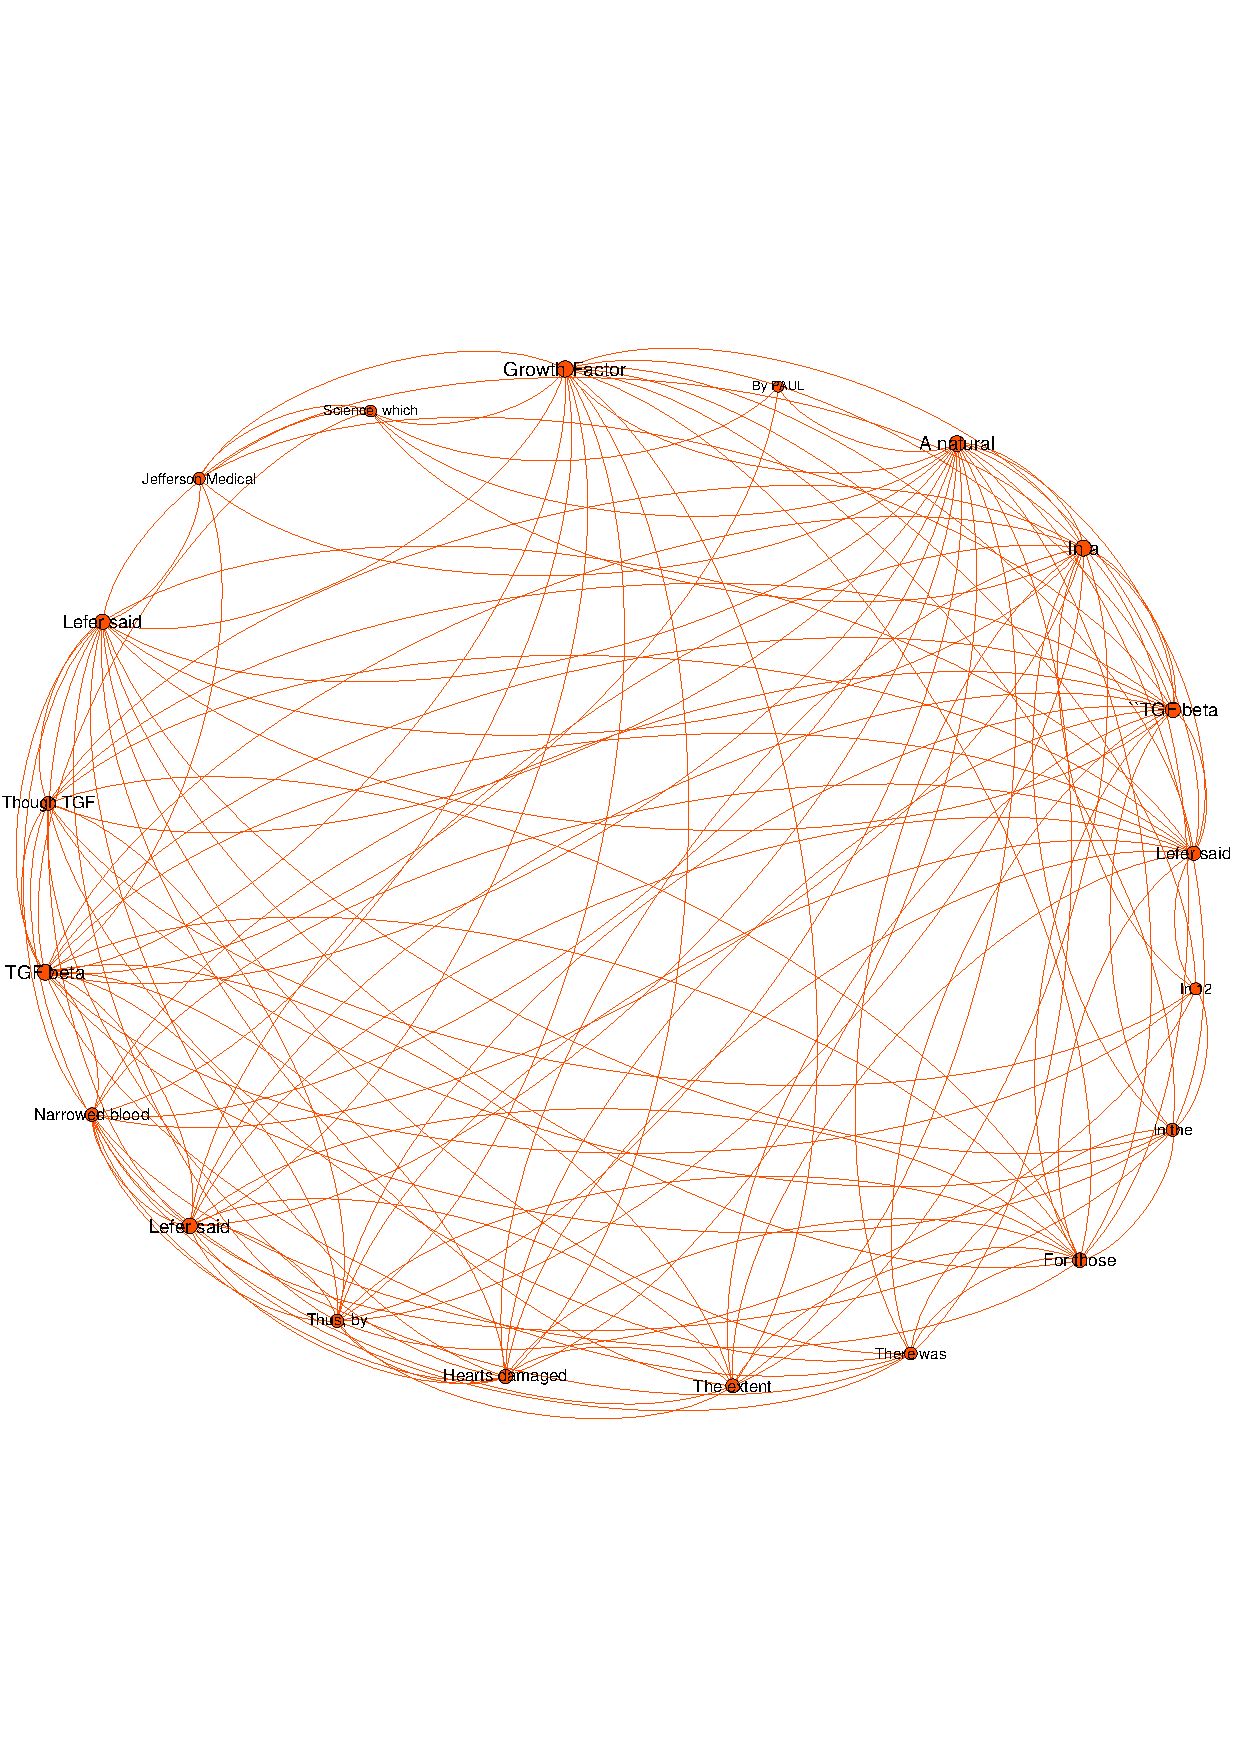
\includegraphics[trim = 0mm 50mm 0mm 50mm, clip, scale=0.15,width=1\textwidth]{Untitled.pdf}
    \caption{Grafo generado a partir del texto.}
\end{figure}

Finalmente, el resumen generado es el siguiente:


% \noindent\fbox{%
%     \parbox{\textwidth}{%
% {\scriptsize
\raisedtext{{\scriptsize \parbox{\linewidth}{A natural substance called transforming growth factor beta appears to be able to limit damage to cardiac cells following a heart attack, according to a study published in the journal Science.
In a study at the Jefferson Medical College in Philadelphia, a group of laboratory rats induced to have heart attacks suffered 50 percent less cell damage after injections of transforming growth factor beta than did rats that did not receive the TGF beta.
Lefer said the TGF beta seems to block the action of other substances, such as tumor necrosis factor, that can cause blood vessels to narrow following a heart attack.
TGF beta is normally present in heart cells, but the study published in Science said that it is missing from rat heart cells damaged by a simulated heart attack.}}}
% \par
% }
%     }%
% }


\section{Variantes propuestas}

En la siguiente sección se describen las variantes que se probaron sobre el algoritmo original de
TextRank. Principalmente estas modificaciones apuntan a cambiar la forma en la cual se calculan las distancias entre las oraciones de los textos. Diferentes métricas arrojaron diferentes resultados y algunas de éstas variantes lograron una mejora significativa sobre el algoritmo original.

\subsection{Subcadena común}
Dadas dos frases, el problema de la subcadena común más larga consiste en identificar la secuencia de caracteres de mayor extensión presente en ambas. Por ejemplo, entre “la cocina verde” y “una cocina vale más si es verde”, la secuencia más larga es “a cocina v”.

La propuesta consiste en modificar la función de distancia de la implementación original y reemplazarla por el largo de la subcadena común más larga. En el ejemplo anterior, la similitud sería de 10, dado que es el largo de la secuencia “a cocina v”.

Cabe destacar el parecido de esta métrica con los métodos de evaluación ROUGE.


\subsection{Similitud coseno}
La similitud coseno es una medida de la similitud existente entre dos vectores en un espacio que posee un producto interior con el que se evalúa el valor del coseno del ángulo comprendido entre ellos. Para poder hacer uso de esta “distancia” se utiliza el modelo vectorial es decir que se modelan a los documentos como vectores.

Este modelo algebraico es utilizado para representar documentos en lenguaje natural de una manera formal mediante el uso de vectores en un espacio multidimensional. La teórica básica es que el parecido de un documento frente a otro puede calcularse usando la similitud coseno. 

Este modelo está basado en favorecer la dirección a la cuál apuntan los documentos independientemente de su longitud. Textos que hablan de los mismos temas pero tienen diferente longitud pueden tener una gran similitud con esta métrica. 

La propuesta se basa en aplicar este modelo para tratar a cada oración del texto como un vector n-dimensional (siendo n la cantidad de palabras distintas presentes en el documento), y luego compararlas utilizando la similitud coseno. Las entradas de cada vector estarán compuestas por el resultado de aplicar la función “frecuencia de término -- frecuencia inversa de documento” (TF--IDF de sus siglas en inglés) a cada palabra de la oración representada.

Tomando como ejemplo el documento “Esta bien. Todo bien.”, las oraciones quedarían modeladas como vectores de la siguiente forma:

\begin{Verbatim}[xleftmargin=3em]
v1=[ TFIDF("Esta") , TFIDF("bien") ,       0       ]
v2=[       0       , TFIDF("bien") , TFIDF("Todo") ]
\end{Verbatim}

Dado que la imagen de la función TFIDF está contenida en el intervalo [0,1], todos los vectores quedan conformados por entradas no negativas, haciendo que ninguna similitud sea menor a cero. 

\subsection{BM25}
Okapi BM25 es una función de ranking utilizada para la asignación de relevancia a los documentos en un buscador. 
Está basada en los modelos probabilísticos de Recuperación de información, y actualmente 
representa el estado del arte en algoritmos de recuperación de documentos basados en frecuencia de término -- frecuencia inversa de documento.

\begin{definicion}
Dadas dos oraciones R, S, BM25 se define como:

\begin{equation}
BM25(R,S) = \sum_{i=1}^{n} IDF(s_i) \cdot \frac{f(s_i, R) \cdot (k_1 + 1)}{f(s_i, R) + k_1 \cdot (1 - b + b \cdot \frac{|R|}{avgDL})}
\end{equation}

donde $k$ y $b$ son parámetros que valen $k = 1,2$ y $b = 0,75$, y $avgDL$ es el largo promedio de las oraciones en el texto.
\end{definicion}

Esta función contempla la frecuencia inversa del documento de manera tal que si una palabra aparece en más de la mitad de los textos, el valor para ese término se vuelve negativo. Dado que este comportamiento no es deseable para esta aplicación, se utiliza la siguiente fórmula:
                
\begin{equation}
 IDF(q_i) =
  \begin{cases}
       log(N - n(q_i) + 0.5) - log(n(q_i) + 0.5)    & \text{si }  n(q_i) > N/2\\
       \varepsilon \cdot avgIDF                     & \text{si }  n(q_i) \leq N/2\\
  \end{cases}
\end{equation}                
                
donde $\varepsilon$ ronda entre 0,5 y 0,30 y $avgIDF$ es el idf promedio para todos los términos.
También se ensayaron alternativas como igualar a cero el resultado en caso de ser negativo, o reemplazar la función inversa por una similar, cuyo resultado es no negativo, o estrictamente positivo. 

Existe una variante a BM25 llamada BM25+. Esta repara deficiencias relacionadas a la frecuencia de término y a la penalización a documentos largos frente a documentos cortos irrelevantes.

La propuesta consistió en aplicar BM25 y BM25+ entre las oraciones de un texto, a fin de ordenarlas de acuerdo a su relevancia.


\subsection{Evaluación}
Se decidió usar la base de datos de la tarea de generación de resúmenes automáticos de la conferencia DUC (Document Understanding Conference) del año 2002 \cite{duc2002-guidelines}. Este el mismo corpus que el usado en la presentación del algoritmo TextRank en \cite{mihalcea-tarau}. El corpus cuenta con 567 documentos que fueron resumidos a cerca del 20\% de su tamaño.

Para llevar a cabo la evaluación se usó la versión 1.5.5 del paquete de métricas ROUGE \cite{Lin2004a}. Se utilizó la configuración usada en DUC, calculando sólo las mediciones ROUGE-1, ROUGE-2 y ROUGE-SU4 en un intervalo de confianza del 95\%. Se obtuvo un único puntaje promediando los tres valores.

Para verificar el funcionamiento de todo el conjunto se desarrolló el método de referencia (\textit{baseline}) usado en \cite{mihalcea-tarau}, que construye el resumen extrayendo las primeras oraciones de cada artículo. Se comprobó que los resultados fueron similares: la versión original de TextRank mejora al \textit{baseline} en un 2,3\% aproximadamente.


\subsection{Resultados Obtenidos}
Los mejores resultados se obtuvieron usando BM25 y BM25+. El incremento más alto se logró al reemplazar los valores negativos por la constante $\varepsilon$ = 0.25, dando una mejora total de 2,92\% para BM25 y 2,60\% para BM25+. Inicialmente se obtuvieron valores cercanos al 1,30\%, pero dado que esta función contempla el uso de \textit{stopwords} se procedió a eliminar la etapa de filtrado del preprocesamiento del texto, alcanzado así resultados sobresalientes. En el Cuadro 1 se detallan las alternativas ensayadas.

\begin{table}
\caption{Resultados de las distintas propuestas}
\begin{center}
\begin{tabular}{l*{5}{c}r}
\hline
\rule{0pt}{12pt}
Método & ROUGE-1 & ROUGE-2 & ROUGE-SU4 & Mejora \\[2pt]
\hline\rule{0pt}{12pt}\mbox{}\par\nobreak
BM25 (Neg a epsilon) & 0.4042 & 0.1831 & 0.2018 & 2,92\% \\
BM25+ (Neg a epsilon) & 0.404 & 0.1818 & 0.2008 & 2,60\% \\
Cosine TF-IDF & 0.4108 & 0.177 & 0.1984 & 2,54\% \\
BM25+ (IDF = log(N/NI)) & 0.4022 & 0.1805 & 0.1997 & 2,05\% \\ 
BM25 (IDF = log(N/NI)) & 0.4012 & 0.1808 & 0.1998 & 1,97\% \\ 
Longest Common Substring & 0.402 & 0.1783 & 0.1971 & 1,40\% \\
BM25+ (Neg a cero) & 0.3992 & 0.1803 & 0.1976 & 1,36\% \\ 
BM25 (Neg a cero) & 0.3991 & 0.1778 & 0.1966 & 0,89\% \\
\textbf{TextRank} & \textbf{0.3983} & \textbf{0.1762} & \textbf{0.1948} & \textbf{--}\\
BM25 & 0.3916 & 0.1725 & 0.1906 & -1,57\% \\
BM25+ & 0.3903 & 0.1711 & 0.1894 & -2,07\% \\
DUC Baseline & 0.39 & 0.1689 & 0.186 & -2,84\% \\ [2pt]
\hline
\end{tabular}
\end{center}
\end{table}

Los tiempos de ejecución también se superaron. Se pudieron procesar los 567 documentos de la base de datos de DUC2002 utilizando 84\% del tiempo requerido por la versión original.

El resultado de la métrica de similitud coseno también fue satisfactoria, presentando una mejora de 2,54\% por sobre el método original. A su vez, los métodos de secuencias de máxima longitud también mostraron una mejora considerable: cerca del 1,40\% por sobre TextRank. En la Figura 1 se comparan los distintas técnicas.

\begin{figure}[h!]
    \centering
    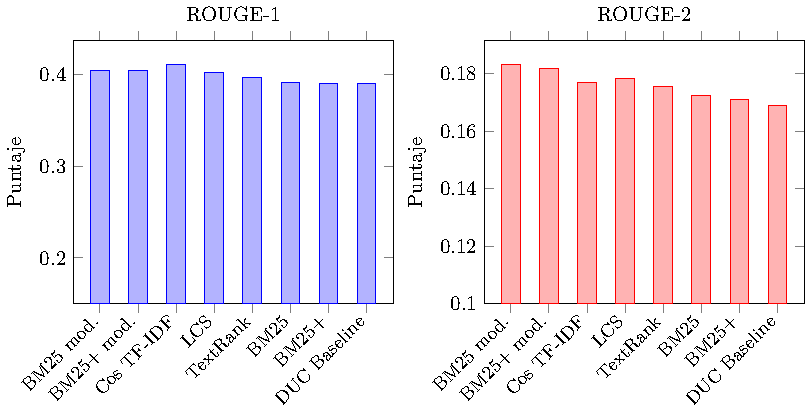
\includegraphics[width=1\textwidth]{rouge-scores.pdf}
    \caption{Comparación de métricas.}
\end{figure}



\section{Conclusiones}
En este trabajo se analizaron variantes al algoritmo de TextRank. A partir del mismo se propusieron e implementaron optimizaciones cuyos resultados fueron significativos: se obtuvo una mejoría del 2,92\% por sobre el método original. Este número es notable si se tiene en cuenta que TextRank por sí solo performa 2,84\% por sobre el estándar de comparación (baseline).

Las evaluaciones fueron hechas con las mismas técnicas y conjuntos de datos utilizados en competencias internacionales, validando así las mediciones.

En base a estos resultados proponemos la utilización de BM25 o BM25+ junto con TextRank como herramienta para la generación de resúmenes automáticos. Los ejemplos analizados y las métricas obtenidas demuestran resultados a los obtenidos por la versión original del algoritmo TextRank sin costo alguno extra de tiempo de procesamiento. 

Queda para próximos trabajos explorar alternativas para la extracción de palabras claves, y el ensayo de distintos métodos algebraicos, haciendo uso del modelo del espacio vectorial.


\bibliography{report}{}
\bibliographystyle{babunsrt}


\end{document}
